\chapter{Convexidad y Optimización}

\section{Introducción}

$$
(P)
\left\{
\begin{array}{rl}
    \min & f_0(x)\\\\
    s.a. & f_1(x) \leq b_1\\
	 &f_2(x) \leq b_2\\
	 & \vdots\\
	 & f_m(x) \leq b_m.
\end{array}
\right.
\qquad
\begin{array}{rl}
    f_i: & \mathbb{R}^n \rightarrow \mathbb{R}\\
    f_0 : & \mbox{Función objetivo.}\\
    f_j : & \mbox{Función Restricción donde }j=1,\ldots,m.\\
\end{array}
$$
\begin{itemize}
    \item Las funciones objetivos en economía se les puede llamar función de coste.
    \item Las desigualdades tiene un truco, si multiplicamos por $(-1)$ tenemos en la forma que decidamos.
    \item Maximizar es lo mismo que minimizar. Por lo que minimizaremos las funciones. 
\end{itemize}

El objetivo de (P) es encontrar $x^*$ el optimo ($\arg\min$) que cumple 
$$f_0(x^*)\leq f_0(x), \;\forall x\in \mathbb{R}^n / f_j(x)\leq b_j,\; j=1,\ldots,m.$$
Será en cualquier $x$ que cumple las restricciones. Los puntos que no cumplen las condiciones no sirven para nada.

Al valor $f_0(x^*)$ se le llama valor optimo.

$f_i:  \mathbb{R}^n \rightarrow \mathbb{R}$ Existirá algunas funciones que su dominio sera tramposo.

Los Puntos factibles son los $x\in \mathbb{R}^n / f_j(x)\leq b_j,\; j=1,\ldots,m.$

\begin{itemize}
    \item  Si los problemas son lineales se llama programación lineal.
    \item Cuando es convexa se llama optimización convexa.
    \item La habilidad es de identificar las restricciones y pasarlas a convexas.
\end{itemize}

\begin{ejem}
Sean $A\in \mathcal{M}_{k\times n},\; \textbf{x}\in \mathbb{R}^n,\; \textbf{b}\in \mathcal{R}^k$.
$$
\begin{pmatrix}
    x_1\\
    x_2\\
    \vdots\\
    x_n
\end{pmatrix}
\in \mathbb{R}^n,
\qquad 
\textbf{x}^T=(x_1,x_2,\ldots,x_n).
$$
Diremos que el un vector cualquiera sera vector columna.

Ahora, el problema será una minimización global dada por:
$$
\left\{
\begin{array}{rl}
    \min: &\|A\textbf{x}-b\|^2_2\\
    s.a. & \emptyset.
\end{array}
\right.
$$

El subindice $_2$ significa la normal Euclidea. Que es la distancia normal que existe en $\mathbb{R}^2.$

El objetivo será encontrar la $x$ donde la operación dada será la menor posible.

\textbf{Nota}
Imaginemos que tenemos 
$$
\begin{array}{rl}
    \left\{\min\right. & f(x)\\\\
    \left\{ \min \right. & f_0^2(x)
\end{array}
$$

Si las función $f_0$ es positiva las dos formas son equivalentes. El valor optimo no será el mismo porque lo estoy elevando al cuadrado, pero el punto optimo lo será. Porque las funciones son monótomas crecientes. Si el valor al cuadrado me simplifica entonces podemos utilizarla. Esto nos permite que si no tengamos una función convexa podamos convexificarla.

Por diferenciabilidad:
$$f_0(x)=\|Ax-b\|_2^2 = \langle Ax-b,Ax-b\rangle.$$


\textbf{Notación.-} Podemos escribir $Ax$ como
$$
Ax = 
\underset{A^1}{
\begin{pmatrix}
    a_{11}\\
    a_{21}\\
    \vdots\\
    a_{k1}
\end{pmatrix}}
x_1+
\underset{A^2}{
\begin{pmatrix}
	a_{12}\\
	a_{22}\\
	\vdots\\
	a_{k2}
\end{pmatrix}}
x_2+
\cdots +
\underset{A^n}{
\begin{pmatrix}
	a_{1n}\\
	a_{2n}\\
	\vdots\\
	a_{kn}
\end{pmatrix}}
x_n
=
x_1A^1+x_2A^2+\cdots+x_nA^n.
$$
$A^1$ = A super 1 como columna, y $A_1$ = A super 1 como fila.

Ahora, en términos de filas. Si escribimos los vectores A en columna
$$
A = 
\begin{pmatrix}
	A^T_1\\
	A^T_2\\
	\vdots\\
	A^T_k
\end{pmatrix}
$$

Donde,
$$
Ax = 
\begin{pmatrix}
	A^T_1x\\
	A^T_2x\\
	\vdots\\
	A^T_nx
\end{pmatrix}
=
\begin{pmatrix}
	\langle A^T_1,x\rangle\\
	\langle A^T_2,x\rangle\\
	\vdots\\
	\langle A^T_n,x\rangle
\end{pmatrix}
$$

Intentaremos demostrar el punto donde las parciales de $f_0=0$. Para ello, encontraremos 
$$
\begin{array}{rcl}
    D_if_0&=&D_i\left(\langle Ax-b, Ax-b\rangle\right)\\\\
	  &=&\langle D_i\left(Ax-b\right),Ax-b\rangle+\langle Ax-b,D_i\left(Ax-b\right)\rangle\\\\
	  &=& 2\langle Ax-b,D_i\left(Ax-b\right)\rangle.
\end{array}
$$

Veamos la parcial de $D_i\left(Ax-b\right)$.
$$
\begin{array}{rcl}
    D_i\left(Ax-b\right)&=&D_i\left(x_1A^1+x_2A^2+\cdots+x_nA^n-b\right)\\\\
			&=&A^i.
\end{array}
$$
Dado que $b$ que es constante vale cero, y donde todos los suman que no estén las $x_i$ también valen cero.

Por lo tanto,
$$D_if_0 = 2\langle Ax-b,A^i \rangle.$$

Luego,
$$2\langle Ax-b,A^i \rangle = 0 \quad \forall i=1,\ldots,n \quad \Rightarrow \quad \langle Ax-b,A^i\rangle=0,\quad \forall i = 1,\ldots,n.$$

Observemos que,
$$
\overrightarrow{0} = 
\begin{pmatrix}
    \langle Ax-b,A^1\rangle\\
    \langle Ax-b,A^2\rangle\\
    \vdots\\
    \langle Ax-b,A^n\rangle
\end{pmatrix}
=
\begin{pmatrix}
    (A_1)^T\\
    (A_2)^T\\
    \vdots\\
    (A_n)^T
\end{pmatrix}
(Ax-b)
=A^T(Ax-b).
$$

En funciones convexas el extremo local será el mínimo global.
$$A^T(Ax-b)=\overrightarrow{0}\quad \Leftrightarrow\quad A^TAx=A^Tb.$$
Que es una ecuación normal.\\

\textbf{Argumentos geométricos}

Sera el mismo calcular el mínimo de la distancia, calcular:
$$\min \|Ax-b\|^2_2 = d(b_i,Ax)^2$$
Donde $Ax$ tendrá la forma geométrica, de un subespacio vectorial. en el caso de $\mathbb{R}^3$ será un plano.
\begin{center}
    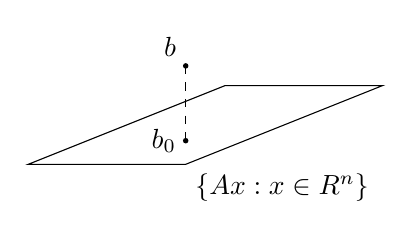
\begin{tikzpicture}[scale=0.5]
      % Define los vértices del romboide
      \coordinate (A) at (0,0);
      \coordinate (B) at (4,0);
      \coordinate (C) at (9,2);
      \coordinate (D) at (5,2);
      % Dibuja el romboide y etiqueta sus vértices
      \draw (A) -- (B) -- (C) -- (D) -- cycle;
      % Que el plano se llame P
      \node [below right] at (B) {$\left\{Ax:x\in \mathbb{R}^n\right\}$};
      % trazar una linea entrecortada perpedicular al plano y los puntos extremos que tengan un punto negro
      \draw[dashed] (4,2.5)node[above left]{$b$} -- (4,.6)node[left]{$b_0$};
      \fill (4,2.5) circle (2pt);
      \fill (4,.6) circle (2pt);
    \end{tikzpicture}
\end{center}

Si $b\in \left\{Ax:x\in \mathbb{R}^n\right\}\quad \Leftrightarrow \quad x^* \in \mathbb{R}^n : Ax^* =b.$ El valor optimo $f_0(x^*)=0.$

Si $b\notin \left\{Ax:x\in \mathbb{R}^n\right\}$, $f_0(x^*)=d(b,b_0)^2$.

Ahora, cual es el optimo?; es decir cual es el $x^*$

Donde la solución es:
$$x^*\in \mathbb{R}^n : Ax^*=b_0.$$ Aquí, $b_0$ está en el plano, si estamos en $\mathbb{R}^3$. ¿Cómo llegamos algebraicamente?:
$$
\begin{array}{rcl}
b-b_0 \perp \left\{Ax:x\in \mathbb{R}^n\right\}&\Leftrightarrow & b-b_o \perp A^i,\; i=1,\ldots,n\\\\  
						 &\Leftrightarrow & \langle b-b_0,A^i\rangle=0,\; i=1,\ldots,n\\\\
							   &\Leftrightarrow& \langle b-Ax^*,A^i\rangle = 0, \; i=1,\ldots,n\\\\
							   &\Leftrightarrow& \langle Ax^*-b,A^i\rangle = 0, \; i=1,\ldots,n\\\\
								   &\leftrightarrow&A^TAx^*=A^Tb.
\end{array}
$$
\end{ejem}
Las ecuaciones normales vienen dadas por la perpendicularidad.

\section{Conjuntos convexos de \boldmath $\mathbb{R}^n$}

El dominio tendrán que ser conjuntos convexos o Dominio efectivo.

% -------------------- DEFINICIÓN 1 LINEAL
\begin{def.}[Lineal]\,\\ 
$$L(x_0,x_1) := \left\{x_0+\lambda(x_1-x_0):\lambda \in \mathbb{R}\right\}$$
\begin{center}
    \begin{tikzpicture}[scale=0.5]
      \coordinate (A) at (0,0);
      \coordinate (B) at (3,1);
      \coordinate (C) at (6,2);
      \coordinate (D) at (-3,-1);
      \draw[->] (A) -- (B)node[below]{$x_1$};
      \draw[dashed] (B) -- (C);
      \draw[dashed] (D) -- (A);
      \fill (A) circle (2pt) node[below]{$x_0$};
    \end{tikzpicture}
\end{center}
\end{def.}

\begin{itemize}
    \item Cuando $\lambda$ vale $1$ me sale $x_1$ cuando valga cero me sale $x_0$ cuando es positivo va hacia la derecha y cuando es negativo va hacia la izquierda.
    \item Toda la recta nos da un concepto que denominamos Afín. 
    \item Para la convexidad no es necesario tener la linea, solo necesitaremos un segmento. 
	$$\left\{x_0+\lambda(x_1-x_0):\lambda \in \left[a,b\right]\right\}$$
    \item El segmento importante será el intervalo que denotaremos como:
	$$\left[x_0,x_1\right]:=\left\{x_0+\lambda(x_1-x_0):\lambda \in \left[0,1\right]\right\}=\left\{(1-\lambda)x_0+\lambda x_1:\lambda \in \left[0,1\right]\right\}$$
	Es cualquier punto que este entre $x_0$ y $x_1$ del gráfico de arriba. 
\end{itemize}


% -------------------- DEFINICIÓN DE AFÍN
\begin{def.}
    Sea $A\subseteq \mathbb{R}^n$. Se dice \textbf{Afín}, si para todo $x, y\in A$ se tiene que la $L(x,y)\subseteq A$. (Subespacios vectoriales desplazados).
\end{def.}

\begin{itemize}
    \item Un circulo no es afín ya que la linea es infinita y un circulo no.
    \item Un plano podría ser Afín
    \item La recta es afín
    \item Todo $\mathbb{R}^n$ es afín.
    \item Un único punto también es afín, dado que $x=y$.
    \item La diferencia entre espacio vectorial y espacio afín es que el espacio afín esta desplazada; es decir, no necesariamente pasa por el cero como en un subespacio vectorial.
\end{itemize}

Manejar el concepto de afín con lineas es un poco incomodo, entonces se utiliza el concepto de combinación afín  

% -------------------- DEFINICIÓN DE combinación afín
\begin{def.}
    Una \textbf{combinación afín} de los vectores $\left\{x_1,x_2,\ldots,x_k\right\}$ es un vector de la forma 
$$\lambda_1 x_1+\lambda_2x_2+\cdots+\lambda_kx_k.$$
tal que 
$$\sum_{i=1}^k \lambda_i = 1.$$
\end{def.}

\begin{itemize}
    \item Lo que decimos que es una combinación lineal de $x_0$ y $x_1$.
    \item Lo demás puntos fuera del segmento son las combinaciones lineales de $x_0$ y $x_1$.
\end{itemize}

% -------------------- TEOREMA 1
\begin{teo}
    $A$ es afín sii $A$ contiene toda combinación afín de sus puntos.

	Demostración.-\; Primero, tomemos puntos arbitrarios $\left\{x_1,x_2,\ldots,x_k\right\}$ en $A$ tal que 
	$$z=\lambda_1x_1+\lambda_2x_2+\cdots+\lambda_kx_k$$
	donde $\sum\limits_{i=1}^k \lambda_i = 1$. 

	Ahora, consideremos dos puntos $x_i,x_j$ de $z$. Dado que $A$ es afín, entonces $L(x_i,x_j)\subseteq A$, para todo $x_i,x_j$. Esto implica que $z$ está en $A$. Intuitivamente, si 
	$$\lambda_1x_1+\lambda_2 x_2,\quad \lambda_3\lambda_3+\lambda_4\lambda_4,\quad \ldots,\quad  \lambda_{k-1}x_{k-1}+\lambda_kx_k$$ 
	están en $A$. Entonces, $z$ tendrá que estar en $A$.

	Para demostrar la otra implicación, tomemos dos puntos cualesquiera $x$ e $y$ en $A$.  Entonces, $L(x,y)\subseteq A$. Por lo tanto, $A$ es afín.
\end{teo}

\begin{itemize}
    \item Quiere decir que este conjunto es estable para combinaciones lineales muy similar al concepto de subespacio vectorial.
\end{itemize}
\vspace{.5cm}

% -------------------- NOTACIÓN 1
\begin{notacion}
La suma de Minkowski es la operación de conjuntos; es decir, si $A,E\subseteq \mathbb{R}^n$. Entonces,
$$A=x_0+E=\left\{x_0+e:e\in E \right\} \quad \mbox{o}\quad E=A-x_0=\left\{a-x_0:a\in A\right\}.$$ 
Es sencillamente trasladar los puntos del plano y desplazarlos o moverlos.
\end{notacion}

\begin{nota}
La definición de subespacio se refiere a tomar dos escalares y dos vectores, realizar la combinación lineal, donde esta combinación lineal no se saldrá del conjunto dado.
\end{nota}


% -------------------- TEOREMA 2
\begin{teo}
    $A\subseteq \mathbb{R}^n$ es afín sii existe un $E\subseteq \mathbb{R}^n$ subespacio vectorial tal que $A=x_0+E$ para todo $x_0\in A$.\\\\
	Demostración.-\; Supongamos que $A$ es afín y fijamos $x_0\in A$. Intentaremos probar que $E=A-x_0$ es un subespacio de $\mathbb{R}^n$, esto es equivalente a decir que:
	$$\lambda,\mu \in \mathbb{R}, e_i,e_2\subseteq E \quad \Rightarrow \quad \lambda e_i+\mu e_2\in E.$$
	Probemos que $\lambda e_1+\mu e_2\in E$; en otras palabras probaremos que $\lambda e_1+\mu e_2$ es $a-x_0$.
	$$
	\begin{array}{rcl}
	    \lambda e_1+\mu e_2&=&\lambda(a_1-x_0)+\mu(a_2-x_0)\\\\
			       &=&\lambda a_1 + \lambda a_2 - \lambda x_0-\mu x_0\\\\
			       &=&\lambda a_1 + \lambda a_2 - \lambda x_0-\mu x_0 +x_0-x_0\\\\
			       &=&\lambda a_1 + \lambda a_2+(1-\lambda-\mu)x_0-x_0.
	\end{array}
	$$
	Observemos que $\lambda a_1 + \lambda a_2+(1-\lambda-\mu)x_0$ está en $A$, dado a que $\lambda+\mu+(1-\lambda-\mu)=1$. Por lo tanto,
	$$A-x_0=E.$$
	Es un subespacio vectorial.

	Ahora, sabemos que $A\subseteq \mathbb{R}^n$ tal que $A=E+x_0$ para todo $x_0\in A$ es afín. Entonces, $E$ es un subespacio vectorial. Para demostrar que $A$ es afín, probaré que cualquier combinación afín de elementos de $A$ sigue estando en $A$. Sean,
	$$\left\{a_1,a_2,\ldots,a_k\right\},\; \lambda_1,\lambda_2,\cdots,\lambda_k:\sum \lambda_i=1.$$
	De donde,
	$$
	\begin{array}{rcl}
	    \lambda_1a_1+\lambda_2a_2+\cdots+\lambda_ka_k&=&\lambda_1(e_1-x_0)+\lambda_2(e_2-x_0)+\cdots+\lambda_k(e_k-x_0)\\\\
							   &=& \lambda_1e_1+\cdots+\lambda_ke_k+\left(\displaystyle\sum_{i=1}^k \lambda_i\right)x_0
	\end{array}
	$$
	Observemos que $\lambda_1e_1+\cdots+\lambda_ke_k$ es una combinación lineal afín el cual existe en $E$ y por definición, $\left(\displaystyle\sum_{i=1}^k \lambda_i\right)=1$. Por lo tanto,
	$$E+x_0=A.$$
\end{teo}

% -------------------- DEFINICIÓN 3 ENVOLTURA O SPAN AFÍN
\begin{def.}[Envoltura Afín]\,\\\\
    La envolura afín de $B$, $Aff(B)$, es el menor conjunto afín que contiene a $B$. Esto implica que es el conjunto de las combinaciones afines de elementos de $B$ o es la intersección de los conjuntos afines que contienen a $B$ 
\end{def.}

% -------------------- DEFINICIÓN
\begin{def.}
    Si $A$ es $Affin$ se llama "dimensión afín de $A$" a la dimensión de su espacio vectorial.
\end{def.}

\begin{itemize}
    \item Dimensión $0$ un punto.
    \item Dimensión $1$ una recta.
    \item Dimensión $2$ una plano.
\end{itemize}



% -------------------- EJEMPLO 2
\begin{ejem}
    Dado $C\in \mathbb{R}^n$ afín. Siempre existirán una matriz $A\in \mathcal{M}_{p\times n}$ y $b\in \mathbb{R}^p$ tal que
    $$C=\left\{x\in \mathbb{R}^n:Ax=b\right\}.$$\\
	Solución.-\; Cuál es el conjunto lineal asociado?, será el núcleo de la aplicación lineal; es decir,
	$$E=\left\{x\in \mathbb{R}^n:Ax=0\right\}.$$
	Cualquier solución de $x_0\in C$, de modo que $Ax_0=b$. Tomando un punto de $C$ y otro de $E$, tenemos 
	$$A(x_0+e)=Ax_0+Ae=b+0=b.$$
	Por lo tanto,
	$$C=\left\{x\in \mathbb{R}^n:Ax=b\right\}=x_0+E.$$
	Así, el conjunto afín no es más que el traslado del espacio vectorial.
\end{ejem}

% -------------------- Definición 1.6
\begin{def.}[Topología de \boldmath$\mathbb{R}^n$]\,\\\\
    Sean $A\subseteq \mathbb{R}^n$ y $a\in \mathbb{R}^n$.
    \begin{enumerate}[1)]
	\item $a\in A$ está en el interior de $A$ $\left(a\in \interior(A) \mbox{ o } \mathring{A} \right)$, cuando existe $\delta>0$ tal que $B(a,\delta)\subseteq A.$
	$$B(a,\delta)=\left\{x\in \mathbb{R}^n:\|x-a\|\leq \delta.\right\}.$$
	Por ejemplo en $\mathbb{R}^2$ será un circulo y $\mathbb{R}^3$ será una esfera.
	\item $A$ se dice abierto si $A=\interior(A)=\mathring{A}.$ (Los puntos frontera del conjunto $A$ serán los abiertos).
	\item Decimos que $c\in\mathbb{R}^n$ está en el cierre (o clausura) de $A$, cuando $\exists \left\{a_n\right\}\in A | a_n\to c$.
	\item Decimos que $A$ es cerrado cuando $A=\overline{A}$ donde $\left\{x\in \mathbb{R}^n: x \mbox{ está en el cierre de }A\right\}.$ (El cierre se divide en los puntos del interior y los puntos frontera).

	\item Se llama frontera de $A$, $\partial{A}$ a la intersección $\overline{A}\cap \left( \overline{\mathbb{R}\backslash A}\right)=\overline{A} \backslash \interior(A)$.
	\item $a\in \relint(A)$ si existe $\delta>0$ tal que $B(a,\delta)\cap Aff(A)\subseteq A$.\\
	    Lo que decimos es que la bola puede ser muy grande y vivir en $\mathbb{R}^3$ e intersecar en el plano, donde se corta transversalmente para proyectar la imagen.
    \end{enumerate}
\end{def.}

\begin{itemize}
    \item El concepto de punto interior será importante, porque me dice que me puedo acercar al punto $a$ desde todas las direcciones, y si es relativo interior me puedo acerca por todos los lados del conjunto.
    \item El punto de adherencia o clausura es un punto que me puedo acercar de alguna forma pero no de todas formas.
\end{itemize}

% -------------------- EJEMPLO 1.3
\begin{ejem}
    Dibujemos un plano
    \begin{center}
      \begin{tikzpicture}[scale=0.5]
	% Define los vértices del romboide
	\coordinate (A) at (-2,0);
	\coordinate (B) at (6,0);
	\coordinate (C) at (11,3);
	\coordinate (D) at (3,3);
	% Dibuja el romboide y etiqueta sus vértices
	\draw (A) -- (B) -- (C) -- (D) -- cycle;
	% Dibuja el contorno del riñón
	\coordinate (Center) at ($(A)!0.5!(C)$);
	\draw[] ($(Center)+(-1,.5)$) .. controls ($(Center)+(0.2,2)$) and ($(Center)+(3,-.1)$) .. ($(Center)+(1,-.4)$) .. controls ($(Center)+(0,-.5)$) and ($(Center)+(0,-1)$) .. ($(Center)+(-1,-.9)$) .. controls ($(Center)+(-1.5,-1)$) and ($(Center)+(-3,-.5)$) .. ($(Center)+(-1,.5)$);
	% Rellena el interior del riñón con líneas
	\pattern[pattern=north east lines, pattern color=gray!50] ($(Center)+(-1,.5)$) .. controls ($(Center)+(0.2,2)$) and ($(Center)+(3,-.1)$) .. ($(Center)+(1,-.4)$) .. controls ($(Center)+(0,-.5)$) and ($(Center)+(0,-1)$) .. ($(Center)+(-1,-.9)$) .. controls ($(Center)+(-1.5,-1)$) and ($(Center)+(-3,-.5)$) .. ($(Center)+(-1,.5)$);
	\node at ($(Center)+(-.2,.2)$) {\small$B$};
	\node at ($(Center)+(1.9,.7)$) {\small$A$};
      \end{tikzpicture}
    \end{center}
    \begin{itemize}
	\item $B$ es el interior con la frontera.
	\item $A$ es la frontera.
	\item El objetivo será encontrar el punto optimo de un esfera que está proyectada en este plano. 
	\item El conjunto tendrá que ser convexo.
    \end{itemize}
    Veamos algunas propiedades de este conjunto.
    \begin{enumerate}[1)]
	\item $A$ es cerrado.- Cualquier punto que ponga en $B$ me puedo acercar por puntos de $B$.
	\item $B$ cerrado.
	\item $\mathring{A}=\emptyset$.- Si yo ponga una bola, se saldrá del conjunto $A$.
	\item $\mathring{B}=\emptyset$.- Ya que no existirá en el plano ninguna esfera. 
	\item $relint(A)=\emptyset$.
	\item $relint(B)=B\backslash A.$
    \end{enumerate}
\end{ejem}

% -------------------- Definición 1.8
\begin{def.}[Combinación convexa]\,\\\\
    Sean $x_1,x_2,\ldots,x_k\in \mathbb{R}^n$ y $\lambda_1,\lambda_2,\ldots,\lambda_k\in \mathbb{R}$ tales que $\lambda_i\geq 0$ y $\displaystyle\sum_{i=1}^{k}\lambda_i=1$. Al vector
    $$\sum_{i=1}^{k}\lambda_ix_i=\lambda_1x_1+\lambda_2x_2+\ldots+\lambda_kx_k$$
    se le llama combinación convexa de los puntos $\left\{x_1,\ldots,x_k\right\}$.\\

	La única diferencia entre combinación convexa y afín es que sean positivos.
\end{def.}

% -------------------- Observación 1.1
\begin{obs}
    La definición para 2 puntos $\left\{x_1,x_2\right\}$ nos de las combinaciones convexas,
    $$\lambda x_1+(1-\lambda)x_2,\qquad \lambda\geq 0, (1-\lambda)\geq 0 \; \Leftrightarrow \; \lambda \in \left[0,1\right].$$
    Esto es el segmento,
    $$\left\{\lambda x_1+(1-\lambda)x_2: \lambda\in \left[0,1\right]\right\}=\left[x_1,x_2\right].$$
    Nos quedamos con el segmento que los une, eso nos permitirá utilizar las propiedades de los números reales. Por lo que podremos realizar análisis.
\end{obs}

% -------------------- Definición 1.9
\begin{def.}[convexo]\,\\\\
    Un conjunto $C\in \mathbb{R}^n$ se dice convexo cuando $C$ contiene las combinaciones convexas de sus puntos, (Decimos que $C$ es cerrado para las combinaciones convexas), si y sólo si
    $$\forall x_1,x_2\in C \Rightarrow \left[x_1,x_2\right]\subseteq C.$$
    Un conjunto es convexo si dados dos puntos el segmento que los une se queda adentro.
\end{def.}

% -------------------- EJEMPLO 1.4
\begin{ejem}
    \begin{multicols}{3}
	\begin{center}
	  \begin{tikzpicture}[scale=0.8]
	    % Dibuja el contorno del riñón
	    \coordinate (Center) at ($(A)!0.5!(C)$);
	    \draw[] ($(Center)+(-1,.5)$) .. controls ($(Center)+(0.2,2)$) and ($(Center)+(3,-.1)$) .. ($(Center)+(1,-.4)$) .. controls ($(Center)+(0,-.5)$) and ($(Center)+(0,-1)$) .. ($(Center)+(-1,-.9)$) .. controls ($(Center)+(-1.5,-1)$) and ($(Center)+(-3,-.5)$) .. ($(Center)+(-1,.5)$);
	    % Rellena el interior del riñón con líneas
	    \pattern[pattern=north east lines, pattern color=gray!50] ($(Center)+(-1,.5)$) .. controls ($(Center)+(0.2,2)$) and ($(Center)+(3,-.1)$) .. ($(Center)+(1,-.4)$) .. controls ($(Center)+(0,-.5)$) and ($(Center)+(0,-1)$) .. ($(Center)+(-1,-.9)$) .. controls ($(Center)+(-1.5,-1)$) and ($(Center)+(-3,-.5)$) .. ($(Center)+(-1,.5)$);
	    % trazar una linea que una dos puntos del contorno pero este fuere del conjunto
	    \draw[dashed](2.6,0.1)--(4,.55);
	    \node at (2.7,-.4) {\small No convexo};
	  \end{tikzpicture}

	  \begin{tikzpicture}[scale=0.7]
	    % Dibuja un óvalo
		\draw (0,0) ellipse (2.5cm and 1.2cm);
		% Agrega un patrón de líneas diagonales al óvalo
		\pattern[pattern=north east lines, pattern color=gray!50] (0,0) ellipse (2.5cm and 1.2cm);
		\node at (0,1.7) {\small Convexo};
	    \end{tikzpicture}

	  \begin{tikzpicture}[scale=0.6]
		\coordinate (A) at (0,0); % Vértice 1
		\coordinate (B) at (2,0); % Vértice 2
		\coordinate (C) at (3,1.73); % Vértice 3
		\coordinate (D) at (2,3.46); % Vértice 4
		\coordinate (E) at (0,3.46); % Vértice 5
		\coordinate (F) at (-1,1.73); % Vértice 6
		\draw (A) -- (B) -- (C) -- (D) -- (E) -- (F) -- cycle; % Dibuja el hexágono
		\draw[pattern=north east lines, pattern color=gray!50] (A) -- (B) -- (C) -- (D) -- (E) -- (F) -- cycle; % Aplica el patrón al hexágono
		\node at (1,4) {\small Convexo};
	    \end{tikzpicture}
	\end{center}
    \end{multicols}
\end{ejem}

Del gráfico 1) ¿Cuál es el menor conjunto convexo que lo contiene?
\begin{center}
  \begin{tikzpicture}[scale=0.8]
    % Dibuja el contorno del riñón
    \coordinate (Center) at ($(A)!0.5!(C)$);
    \draw[red] ($(Center)+(-1,.8)$) .. controls ($(Center)+(0.2,2)$) and ($(Center)+(3,-.1)$) .. ($(Center)+(1,-.5)$) .. controls ($(Center)+(0,-.8)$) and ($(Center)+(0,-1)$) .. ($(Center)+(-1,-.9)$) .. controls ($(Center)+(-1.5,-1)$) and ($(Center)+(-3,-.5)$) .. ($(Center)+(-1,.8)$);
    % Rellena el interior del riñón con líneas
    \pattern[pattern=north east lines, pattern color=gray!50] ($(Center)+(-1,.5)$) .. controls ($(Center)+(0.2,2)$) and ($(Center)+(3,-.1)$) .. ($(Center)+(1,-.4)$) .. controls ($(Center)+(0,-.5)$) and ($(Center)+(0,-1)$) .. ($(Center)+(-1,-.9)$) .. controls ($(Center)+(-1.5,-1)$) and ($(Center)+(-3,-.5)$) .. ($(Center)+(-1,.5)$);
    % trazar una linea que una dos puntos del contorno pero este fuere del conjunto
  \end{tikzpicture}
\end{center}

% ------------------- Definición 1.10
\begin{def.}
    se llama Envoltura convexa de $A$ al menor conjunto convexo que lo contiene $\Leftrightarrow$ la intersección de todos los convexos que contienen a $A$, denotado por $co(A)$.
    Es equivalente a decir que
    $$co(A)=\left\{\mbox{Combinación convexa de puntos de A.}\right\}$$
\end{def.}

% ------------------- Ejercicio 
\begin{ejer}
    Demostrar que la intersección de conjuntos convexos es convexo.\\\\
	Demostración.-\; 
\end{ejer}


% ------------------- Definición 1.11
\begin{def.}[Cono]\,\\\\
    Un conjunto $C\subseteq \mathbb{R}^n$ se llama cono si y sólo si
    $$\lambda x\in C \mbox{ si } x\in C,\; \lambda \geq 0.$$

    Contiene los rayos que pasan por el cero e intersecan a un punto dado.
    \begin{itemize}
	\item Un cono siempre contiene al origen.
	\item La envoltura cónica de un conjunto es $con(A)=\left\{\lambda : \lambda \geq 0, a\in A\right\}$ la intersección de todos los conos que contiene a $A$.
	\item Un cono $C$ es convexo si y sólo si 
	$$\lambda_1,\lambda_2\in C \Rightarrow \lambda_1x_1+\lambda_2x_2\in C, \; \forall \lambda_1,\lambda_2 \geq 0.$$
    \end{itemize}
\end{def.}

El hiperplano es un caso particular del estudio convexo.

% ------------------- Definición 1.12
\begin{def.}[Hiperplano]\,\\\\
    $H\subseteq \mathbb{R}^n$ es un \textbf{hiperplano} si existe $a\in \mathbb{R}^n \backslash\left\{0\right\}$ tal que
    $H=\left\{x\in \mathbb{R}^n : \langle a,x\rangle = a^T x = 0\right\} = a^\perp$
\end{def.}

% ------------------- 
